\subsubsection{Alloy Design}
%\begin{figure}
%	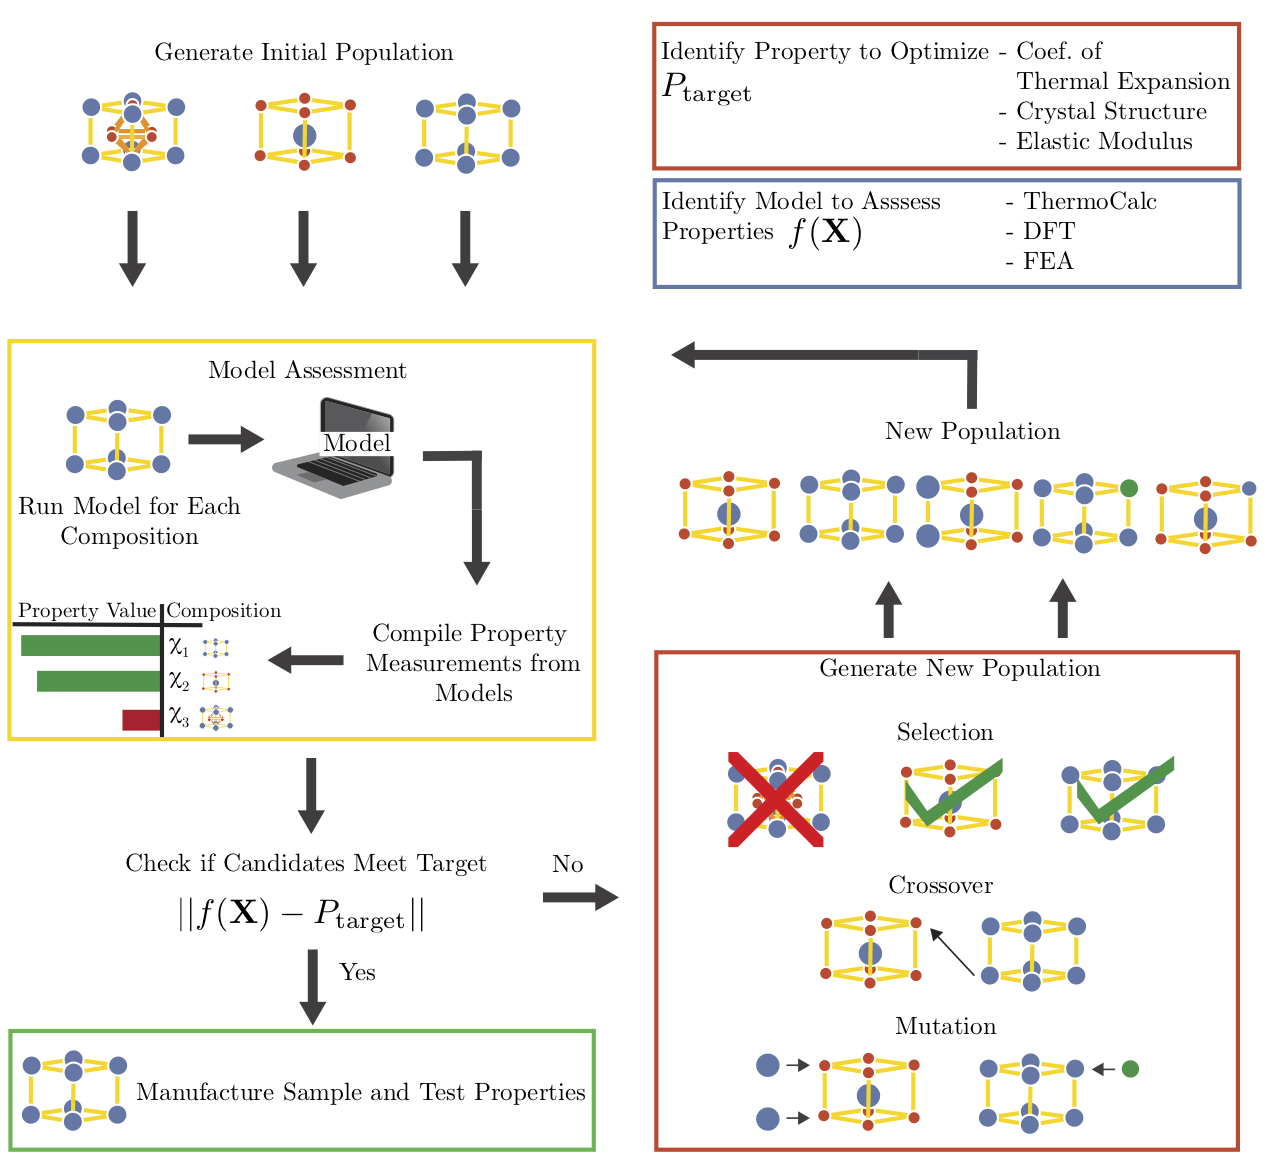
\includegraphics[width=1\linewidth]{Images/AlloyDesign}
%	\caption{}
%	\label{}
%\end{figure}
Choice of alloy impacts the physics of AM from start to finish, starting with the optics of energy sources incident on feedstock and ending with the material properties of the final part. For example, the reflected/absorbed intensity of lasers on powder beds is determined by the powder's composition \cite{Boley2016, Trapp2017}. The density of feedstock, both intra- and inter-granular density, plays a role in final part density \cite{Bi2013}. Conduction modes in the melt are partially determined by the thermal properties of the alloy \cite{Martin2017}. All of this is not to mention that different alloys exhibit different solidification kinetics, which can lead to drastically different microstructures after manufacture \cite{Collins2016}. 

Problems in the additive process can also be linked to composition such as vaporization of constituent elements due to rapid thermal fluxes, impacting the stoichiometry of melt pools and, ultimately, quality \cite{Brice2018}. Traditional engineering alloys sometimes need to be altered to improve compatibility with AM. Searching for new alloys specifically for AM may also be fruitful, as unique strengthening mechanisms can arise \cite{Brice2018, Wang2017}. Designing alloys for AM -- either altering currently used alloys or starting from scratch -- requires taking into consideration the compatibility of alloys' physical properties with AM. Alloy design for AM must take into consideration general alloy properties, like melting point, to feedstock-level properties, like vaporization temperature, to bulk alloy properties, like strength. Much of this information has been collated into databases that are compatible with design for AM. Alloy designers from AM should take advantage of these databases to search for new alloys for use in additive. 

Databases exist that contain alloy properties ranging from the reflectivity of the alloy to the mechanical properties of alloys in bulk. The International Crystal Structure Database (ICSD) contains crystallographic information for millions of compositions. The Linus Pauling files contains a range of material information, from atomic properties like radius and electron valency to crystallographic level information \cite{Villars1998}. In modern day, large databases such as AFLOWLib \cite{Curtarolo2012a}, the Materials Project \cite{Jain2013} and more allow users to search through large databases of relevant alloy information to find one that matches a desired property. Searching through large databases of information to find optimal compositions for manufacturing is actually one of the earliest materials informatics problems ever addressed. Methods exist to perform these searches in a fast, automated way. These methods are referred to as database mining, a data-driven materials design approach.

A study by Martin et al. used database mining to find micronucleants for Al alloys in powder bed manufacturing \cite{Martin2017}. Part of the design process is identifying which alloy properties are important for the desired application. Heterogeneous nucleation of Al grains was the desired outcome of Martin's study. To induce such nucleation, Martin et al. searched for possible nucleants whose crystallographic lattice parameters closely matched that of Al. This way, the Al grains would have a low-energy-barrier nucleating site from which to grow heterogeneously. Martin's study employed a search algorithm to search through 4,500 different possible nucleants and identify those with the closest-matching parameters. Ultimately, Zr was found to be the best candidate.

The same process employed by Martin -- identify the properties which need to be satisfied, then search for a material that is closest matching -- can be extended to many other alloy properties relevant to AM. Database mining was first introduced in material science to predict stable compositions, or estimate material properties from composition. Database mining has been successfully implemented to predict stable crystal structures \cite{Franceschetti1999, Fischer2006, Oganov2006} and predict material properties as a function of composition \cite{Ikeda1997, Gopakumar2018, Wu2018, Kirklin2013, Setyawan2011}. Some specially designed search algorithms have also been designed for improved speed in automated searches \cite{Wolf2000}. Successes have been found in designing Heusler compounds using high throughput search methods \cite{Roy2012}. Reviews of early high-throughput searches for compositions with ideal properties can be found in \cite{Gilmer1998, Koinuma2004}. The same search algorithms employed in these studies can be extended to the additive case.

A limiting factor in database mining is that designers are limited to properties which have been measured or calculated. We do not have information about the vast space of \textit{possible} materials. Consider a set of alloying elements for Ti such as $\{\text{Al}, \text{V}, \text{Zr}, \text{Cr}\}$. Researchers may need to test the impact of alloying composition on the dendrite arm spacing of Ti alloys. Phase field models exist which simulate the growth of and measure dendrite arm spacing as a function of a continuum of composition. A particularly efficient combined phase field/cellular automata model was implemented by Tan et al. precisely to model dendrite arm spacing in laser manufactured alloys \cite{Tan2011}. 

Modeling all possible combinations of $\{\text{Ti},\text{Al}, \text{V}, \text{Zr}, \text{Cr}\}$ is possible with coarse additions of alloying elements, but undesirable. Machine learning can aid in the process to find an optimal composition without modeling all possibilities. \textit{Genetic alogrithms} (GA) can search the space of possible alloys to find the optimal dendrite arm spacing. Genetic algorithms have been one of the most-used data driven approaches in materials science over the past few decades \cite{Morris1996, Ho1998, Wolf2000, Johannesson2002, Stucke2003, Hart2005, Oganov2006}.

The principle of genetic algorithms is to evaluate the \textit{fitness} of a population of candidate alloys against a \textit{fitness function}. The fitness function is a method of evaluating how well a candidate alloy meets a criteria.

As a thought experiment, consider using the CALculation of PHase Diagrams (CALPHAD) method as a fitness function. It can be run for candidate compositions -- in this case, various amounts of $\{\text{Al}, \text{V}, \text{Zr}, \text{Cr}\}$ alloyed into Ti -- and used to evaluate its compatibility with rapid solidification. This is similar to a study completed in \cite{Li2017}. Once a fitness function has been identified, the next step in a genetic algorithm is to represent candidate alloys as a \textit{gene}. 

We can represent a gene as \\

% You must have an empty line between text and the start of a table for some reason -- this is definitely going to be a problem later
\begin{table}[h!]
\begin{tabular}{cccccc}
	Alloy & $=$ & [$\chi_1$, & $\chi_2$, & $\ldots$, & $\chi_n$] \\
\end{tabular}
\end{table}
where $\chi_1$ is the species and weight percent of the first element (titanium, in this example), $\chi_2$ is the species and weight percent of the second element, up to $n$ elements. For example, Ti-6Al-4V would be represented as \\

\begin{table}[h!]
\begin{tabular}{ccc}
	 [0.9 Ti,  & 0.06 Al, & 0.04 V ] \\
\end{tabular}
\end{table}
The goal is to find the alloy with optimal dendrite arm spacing. First, a population of candidate genes needs to be generated, either randomly or by design. Two examples from a starting population may be \\

\begin{table}[h!]
\begin{center}
\begin{tabular}{ccccc}
	Alloy 1 & $=$ & [0.9 Ti, & 0.05 Al, & 0.05 V ] \\
	Alloy 2 & $=$ & [0.9 Ti, & 0.1 Zr] & \\
\end{tabular}
\end{center}
\end{table}
The thermodynamic properties of the various compositions, and therefore their compatibility with AM, is estimated by running a CALPHAD model for each composition. It is not guaranteed that the optimal composition is in this starting population.

Genetic algorithms select genes out of the current population -- called the parent generation --  to proceed to another generation of model assessment -- called the child generation. Selection consists of keeping the best performing compositions, say the top $10\%$, and discarding the rest. Genetic algorithms find optimal locations in the design space by relying on the similarity hypothesis. If one alloy is in the top $10\%$ of genes then it is possible that a similar alloy will also be high performing -- it may be even perform better. Once selection is done, the next step is to search the space near the best performing alloys from the parent generation.

Genetic algorithms generate similar compositions from those selected in the parent generation by making alterations to genes. One operation is \textit{mutation}, whereby entries of the genes are changed. For example, we could mutate alloy 1 by changing the composition:

\begin{table}[h!]
\begin{center}
\begin{tabular}{c|ccccc}
	\textbf{Parent Generation:} & Alloy 1 & $=$ & [0.9 Ti, & {\color{red}0.05} Al, & {\color{red}0.05} V ] \\ \hline
	\textbf{Child Generation:} & Alloy 1 & $=$ & [0.9 Ti, & {\color{green}0.02} Al, & {\color{green}0.08} V  ]  \\ 
\end{tabular}
\end{center}
\end{table}
\noindent where in the child generation the amount of V was increased, while the amount of Al was decreased. Another operation which may be performed is \textit{crossover} where entries of genes are added or interchanged. For example, one crossover operation may look like

\begin{table}[h!]
\begin{center}
\begin{tabular}{c|ccccc}
	\textbf{Parent Generation:} & Alloy 1 & $=$ & [0.9 Ti, & 0.05 Al, & 0.05 {\color{red} V} ]  \\
						 & Alloy 2 & $=$ & [0.9 Ti, & 0.1 {\color{green} Zr}] &              \\ \hline					 
	 \textbf{Child Generation:} & Alloy 1 & $=$ & [0.9 Ti, & 0.05 Al, & 0.05 {\color{green} Zr} ]  \\
						& Alloy 2 & $=$ & [0.9 Ti, & 0.1 {\color{red} V}] &              \\ 
\end{tabular}
\end{center}
\end{table}
\noindent where in the second generation V and Zr have been interchanged.

Selection, mutation, and crossover followed by model assessment and further selection, mutation, and crossover continues until the design criteria is met. The intuition behind genetic algorithms is that eventually the selection process is narrowed down to alloys within a given region of the design space such that further mutation and crossover do not produce new genes. Eventually, all the `fittest` genes as determined by the model will converge to be approximately the same composition. 

Genetic algorithms have been applied to alloy design for low and high temperature structural materials \cite{Ikeda1997, Kulkarni2004}, ultra high strength steels \cite{Xu2008}, specific electronic band gaps \cite{Dudiy2006}, minimum defect structures \cite{Anijdan2006}, exploring stable ternary or higher alloys alloys \cite{Hautier2010, Johannesson2002}, and more. For a review on the application of GA's to alloy design through the early 2000s see Ref. \cite{Chakraborti2004}.

Other machine learning algorithms have also been applied for classification and optimization of alloy compositions. Anijdan used a combined genetic algorithm--neural network method to find Al-Si compositions of minimum porosity \cite{Anijdan2006}. Liu et al. applied partial least squares to data mining of structure-property relationships across compositions \cite{Liu2006}. Decisions trees have been implemented for a number of different alloy optimization, such as predicting ferromagnetism \cite{Landrum2003} and the stability of Heusler compounds \cite{Oliynyk2016}. 
 
In the search for new alloys, some compositions definitely \textit{won't} be compatible with the additive process. It would be useful to identify these alloys up front or as quickly as possible. Additive can also be improved by machine learning algorithms which suggest the best materials or properties to test. A wide range of machine learning algorithms can be implemented to guide the entire experimental design process so that an optimized property is found as quickly as possible. 